\documentclass[12pt]{article}

\usepackage[utf8]{inputenc}
\usepackage[english, russian]{babel}

\usepackage{slides}

\IfFileExists{cyrtimes.sty}
    {
        \usepackage{cyrtimespatched}
    }
    {
    }

\usepackage{graphicx}
\def\Student{Романов Алексей Сергеевич}
\def\Advisor{Рудаков Игорь Владимирович}
\def\Title{Анализ UML диаграмм деятельности с помощью раскрашенных сетей Петри}
% Титул для нижнего колонтитула. Может быть сокращённым
\def\FooterTitle{\Title}
\def\SubTitle{Дипломная работа}
\newcommand{\TitleSlide}{
    \addcontentsline{toc}{section}{\Title}%
    ~\vspace{1cm}

    \begin{center}
    {\huge \begin{spacing}{1}\Title\end{spacing}}

    {\SubTitle}
    \vspace{2cm}

    \ifthenelse{\isundefined{\Student}}{}
        {\small Студент: \Student\\}
    \ifthenelse{\isundefined{\Advisor}}{}
        {\small Руководитель: \Advisor\\}
    \ifthenelse{\isundefined{\Person}}{}
        {\Person\\}
    \ifthenelse{\isundefined{\Affilation}}{}
        {\Affilation\\}
    \end{center}
    \thispagestyle{empty}
}


%% Переносы в презентации смотряся не очень.
\hyphenpenalty 10000
\sloppy


\begin{document}

\TitleSlide

\section{Цели и решаемые задачи}

\emph{Целью работы} является исследование, разработка и реализация метода представления диаграммы деятельности в виде раскрашенной сети Петри, позволяющего выявить блокировки и недостижимые состояния.

\emph{Решаемые задачи}

\begin{enumerate}
\item[1.] Провести обзор и классификацию существующих методов анализа диаграмм деятельности.
\item[2.] Разработать метод представления диаграммы деятельности в виде раскрашенной сети Петри.
\item[3.] Программно реализовать предложенный метод.
\item[4.] Исследовать факторы, влияющие на появление блокировок.
\end{enumerate}

\section{Классификация методов анализа диаграмм деятельности}

\begin{enumerate}
\item[1.] Автоматные методы анализа.
\item[2.] Простая сеть Петри.
\item[3.] Исполняемый UML.
\item[4.] Раскрашенная сеть Петри.
\end{enumerate}

\section{Функциональная модель системы}

\begin{center}
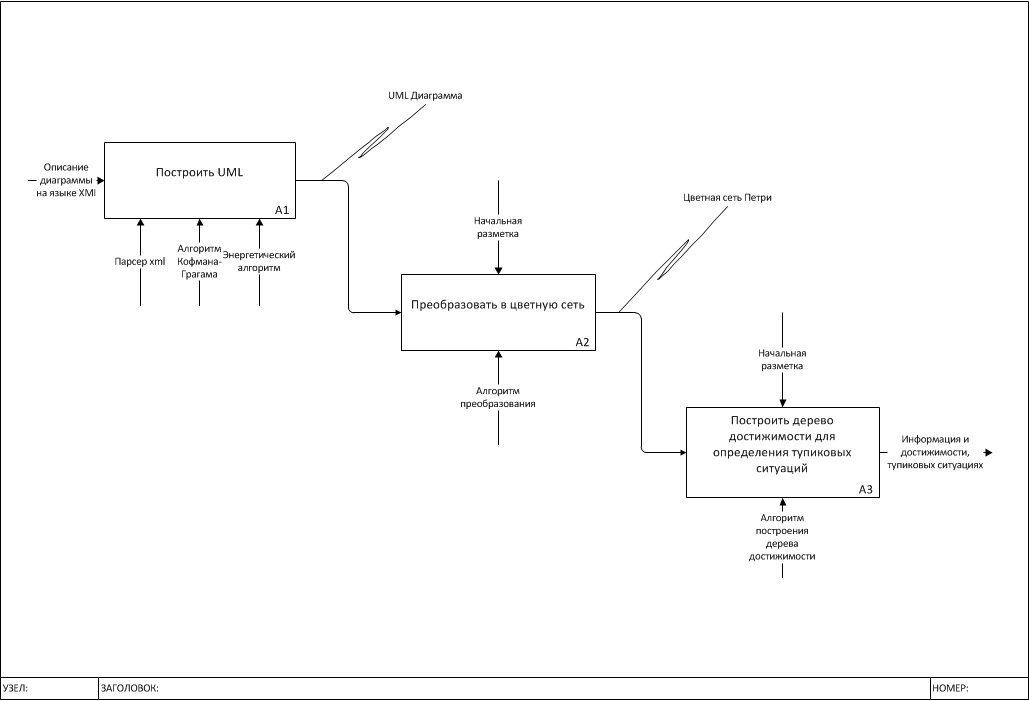
\includegraphics[width=\textwidth]{../tex/include/IDEF0.png}
\end{center}

\section{Представление UML диаграмм}

\begin{minipage}[H]{0.4\linewidth}
Основным стандартом для представления UML диаграмм является XMI (XML metadata interchange) – стандарт OMG для обмена метаданными с помощью языка XML.
\end{minipage}
\hfill
\begin{minipage}[H]{0.60\linewidth}
	\begin{small}
		\begin{verbatim}
<activity_diagram>
    <states>
        <state id, name, type>
            <incoming transitions>
            <outgoing transition>
            <action>
        </state>
    </states>
    <transitions>
        <transition id>
            <source state>
            <target state>
            <guard>
        </transition>
    </transitions>
<activity_diagram>
		\end{verbatim}
	\end{small}
\end{minipage}

\section{Отображение диаграммы деятельности}

Представим диаграмму деятельности в виде ориентированного графа. Тогда для ее отображения будем использовать алгоритм полилинейного изображения планарного графа. Алгоритм состоит из трех этапов.
\begin{enumerate}
\item[1.] Построение ассоциированного орграфа.
\item[2.] Топологическая сортировка вершин исходного и ассоциированного графа.
\item[3.] Мозаичное и полилинейное представление.
\end{enumerate}

\section{Построение ассоциированного орграфа}

Определим ассоциированный орграф G* следующим образом:
\begin{itemize}
\item вершинами графа являются элементы множества граней исходного графа;
\item для любой дуги $ e $ в исходном графе, определим дугу $ e^{*} = (f, g) $ в ассоциированном графе $ G^{*} $, где $ f $ ~--- левая по отношению к $ e $ грань, а $ g $ ~--- правая.
\end{itemize}

Для построения G* необходимо получить список всех граней графа. Под гранью будем понимать простой цикл графа, не содержащий в себе других циклов. 

\section{Мозаичное представление графа}

\begin{minipage}[H]{0.49\linewidth}
	\center{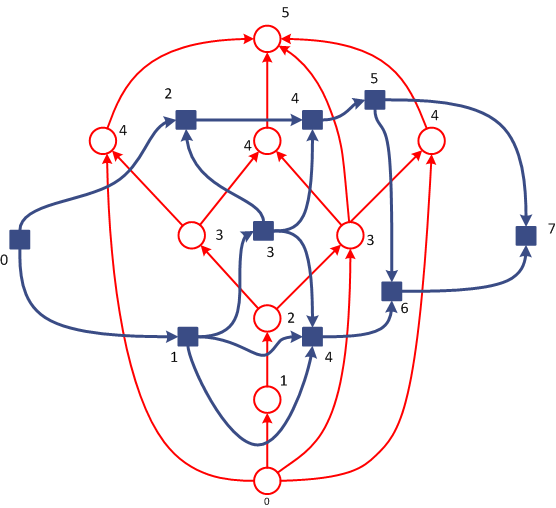
\includegraphics[scale=0.9]{../tex/include/Graph.png}}
	\caption{\begin{small}Исходный граф и ассоциированный орграф G*.\end{small}}
\end{minipage}
\hfill
\begin{minipage}[H]{0.49\linewidth}
	\center{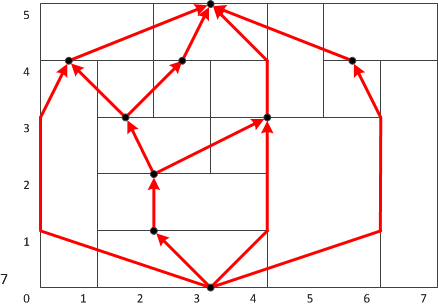
\includegraphics[scale=0.9]{../tex/include/PolylineView.png}}
	\caption{\begin{small}Полилинейное представление графа.\end{small}}
\end{minipage}

\section{Раскрашенные сети Петри}

Раскрашенная сеть Петри представляет собой направленный граф с двумя типами вершин ~--- \textbf{позициями} и \textbf{переходами}, при этом дуги не могут соединять вершины одного типа, т.е. граф является двудольным.

\emph{Отличия раскрашенных сетей от простых сетей Петри}

\begin{itemize}
\item Каждая позиция имеет свой цвет и определяет тип фишек, которые могут там находиться.
\item Каждый переход может иметь спусковую функцию, ограничивающее движение фишек.
\item Для манипуляции цветом применяются функции и переменные, цвет переменной может меняться при прохождении перехода.
\end{itemize}

\section{Этапы построения раскрашенной сети Петри}

\begin{center}
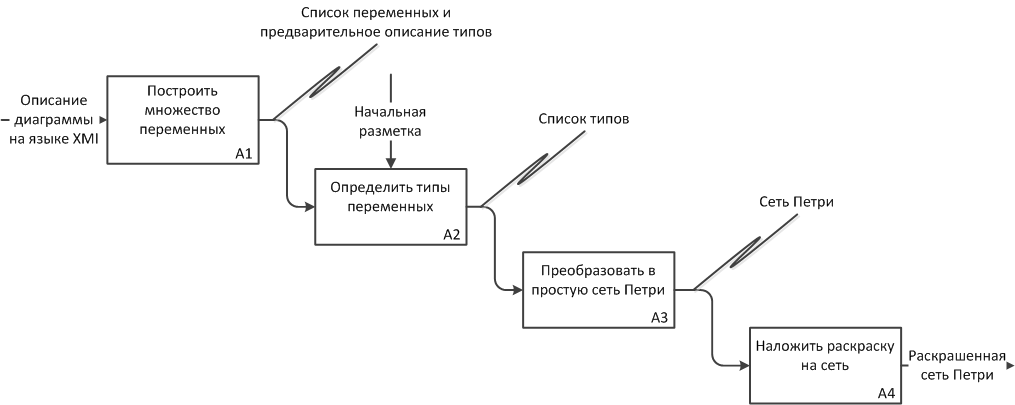
\includegraphics[width=\textwidth]{../tex/include/IDEF0ColoredPetri.png}
\end{center}

\section{Преобразование диаграммы деятельности в раскрашенную сеть Петри}

\begin{minipage}[H]{0.55\linewidth}
	\center{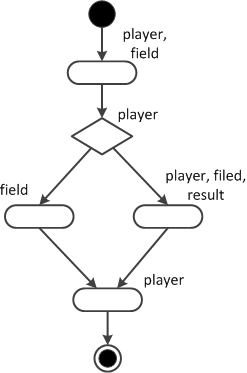
\includegraphics[scale=1.3]{../tex/include/ConvertVariables.png}}
\end{minipage}
\hfill
\begin{minipage}[H]{0.44\linewidth}
Выделение списка переменных для каждой вершины.
\end{minipage}

\section{Преобразование диаграммы деятельности в раскрашенную сеть Петри}

\begin{minipage}[H]{0.55\linewidth}
	\center{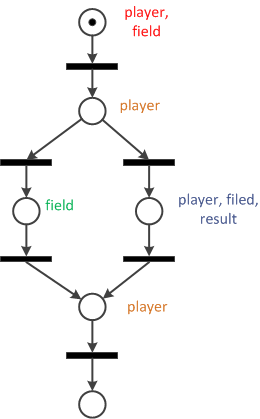
\includegraphics[scale=1.3]{../tex/include/ConvertDiagram.png}}
\end{minipage}
\hfill
\begin{minipage}[H]{0.44\linewidth}
Преобразование диаграммы деятельности в простую сеть Петри и формирование множества типов для соответствующих переменных. Предварительное определение множества раскрасок.
\end{minipage}

\section{Преобразование диаграммы деятельности в раскрашенную сеть Петри}

\begin{minipage}[H]{0.55\linewidth}
	\center{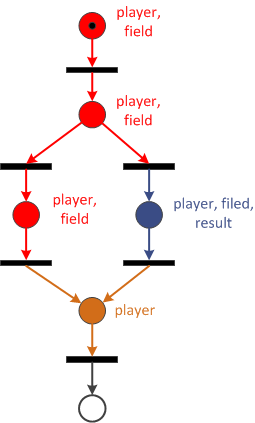
\includegraphics[scale=1.3]{../tex/include/ConvertColoring.png}}
\end{minipage}
\hfill
\begin{minipage}[H]{0.44\linewidth}
Определение максимальной области видимости переменных и формирование результирующей раскраски.
\end{minipage}

\section{Проведенные исследования}

В диаграммах деятельности блокировки могут возникать по причине:

\begin{itemize}
\item неверной структуры диаграммы;
\item невозможности перехода из-за невыполнения логичского условия спусковой функции.
\end{itemize}

\begin{minipage}[H]{0.49\linewidth}
	\center{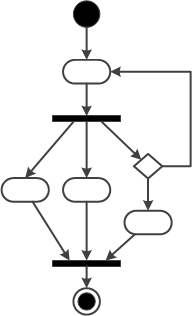
\includegraphics[scale=1]{../tex/include/BlockedDiagram1.png}}
\end{minipage}
\hfill
\begin{minipage}[H]{0.49\linewidth}
	\center{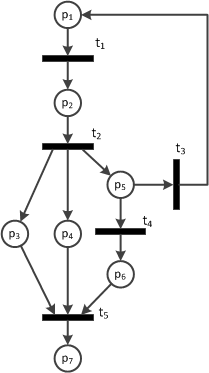
\includegraphics[scale=1]{../tex/include/BlockedNet1.png}}
\end{minipage}

\section{Проведенные исследования}

\begin{minipage}[H]{0.49\linewidth}
	\center{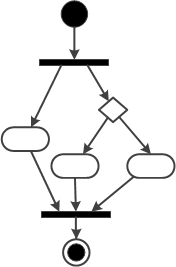
\includegraphics[scale=1]{../tex/include/BlockedDiagram2.png}}
\end{minipage}
\hfill
\begin{minipage}[H]{0.49\linewidth}
	\center{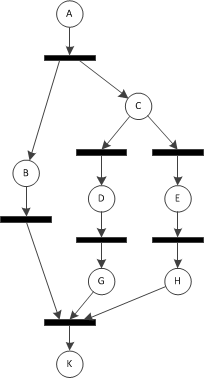
\includegraphics[scale=1]{../tex/include/BlockedNet2.png}}
\end{minipage}



\section{Выводы}

\begin{enumerate}
\item[1.] Проведен оброз существующих методов анализа диаграмм деятельности и осущствленно их сравнение по набору критериев.
\item[2.] Разработан метод представления диаграммы деятельности в виде раскрашенной сети Петри.
\item[3.] Разработано программное обеспечение, реализующее предложенный метод.
\item[4.] Исследованы факторы, влияющие на точность и правильность представления диаграммы в виде раскрашенной сети Петри.
\end{enumerate}

\end{document}

